\section{Complex geometries}
\label{sec:md_complex_geometries}
As we did with DSMC, we want to study flow in arbitrary geometries.  To be able to do this, we need to create a model that satisfies some properties we already have in DSMC. The flowing fluid needs to
\begin{itemize}
	\item be confined in a subset of the total volume,
	\item have realistic interactions with the solid wall, and
	\item have energy drained by the solid.
\end{itemize}
The first requirement is not completely strict, but most of the flowing fluid should be in the free volume. The reason why we need to drain the energy is that in order to induce fluid flow, we apply a constant force that increases the total energy of the system. We want to reach an equilibrium where the average rate of drained energy exactly matches the energy added by the applied force. We assume that the geometry is described as a boolean function $G : \mathbb{R}^3\rightarrow \{1,0\}$ that fully determines whether a point in space is part of the solid or the free volume. A convenient representation is the voxelization described in section \ref{sec:dsmc_binary_representation}. 
\subsection{A naive approach}
To illustrate the basic idea, we will discuss the simplest model satisfying only the first two requirements. Given a molecular dynamics state, we can loop through the positions $\vec r_i$ of each atom $i$, and mark the atoms as \textit{frozen} if $G(\vec r_i) = 1$ (which means that this point is part of the solid). Atoms marked as frozen will not move at all, but all forces are calculated normally. One way of interpreting the non-moving frozen atoms is that they have infinite mass. The total energy is still conserved in the system. An implementation is illustrated in listing \ref{lst:md_simple_solid}.

\begin{lstlisting}[caption=Example code showing how to mark atoms within a solid., label=lst:md_simple_solid]
bool point_is_a_solid(Vector3 &position) {
	int voxel_index_i = position.x / system_length.x * num_voxels.x;
	int voxel_index_j = position.y / system_length.y * num_voxels.y;
	int voxel_index_k = position.z / system_length.z * num_voxels.z;

	// The world matrix is a binary matrix
	return world_matrix[voxel_index_i, voxel_index_j, voxel_index_k];
}

void mark_frozen_atoms() {
	for(int i=0; i<number_of_atoms; i++) {
		Vector3 &position = positions.at(i);
		if(point_is_a_solid(position)) {
			atom_types.at(i) = FROZEN;
		}
	}
}

void move() {
	for(int i=0; i<number_of_atoms; i++) {
		if(atom_types.at(i) != FROZEN) {
			// Only move non-frozen atoms
			positions.at(i).x += velocities.at(i).x*dt;
			positions.at(i).y += velocities.at(i).y*dt;
			positions.at(i).z += velocities.at(i).z*dt;
		}
	}
}
\end{lstlisting}
If the atoms forming the solid are dense enough, very few atoms will be inside the wall, so the first requirement is satisfied. The interaction between the solid and the flowing fluid is as realistic as the potential is, so the only requirement not satisfied is the drainage of the energy. In figure \ref{fig:md_simple_solid}, we see how the red flowing atoms are confined within a cylinder with some radius $R$. 

\begin{figure}[h]
\begin{center}
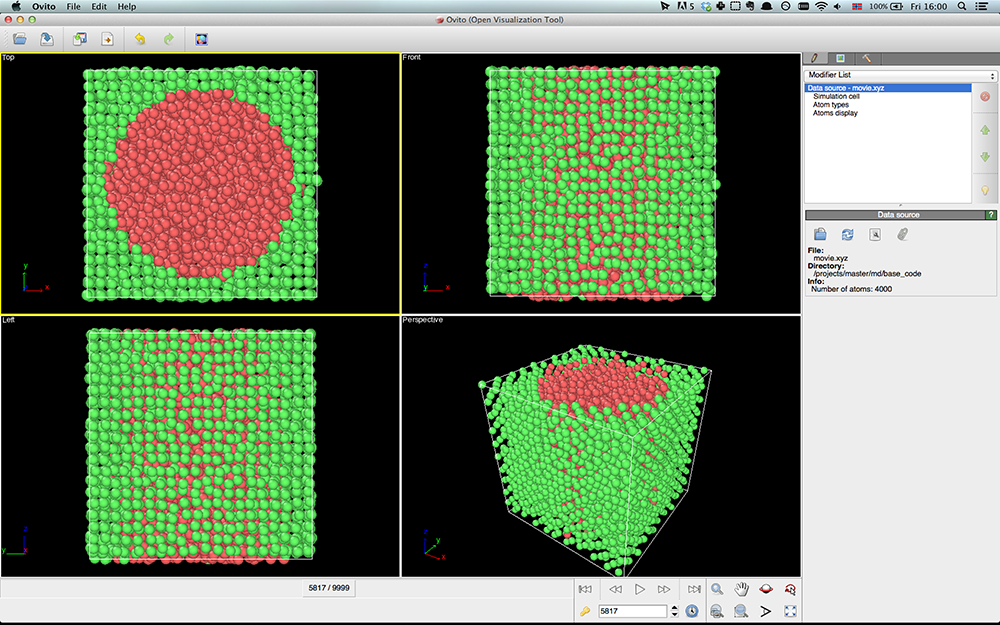
\includegraphics[width=1.0\textwidth, trim=0cm 0cm 0cm 0cm, clip]{MD/figures/solid_model.png}
\end{center}
\caption{A naive model of a solid where the green atoms are completely frozen confining the red flowing atoms within a cylinder of radius $R$. The visualization is done in Ovito, an open source visualization tool.}
\label{fig:md_simple_solid}
\end{figure}

\subsection{A simple model of a solid}
\label{sec:md_simple_model_of_a_solid}
We can improve the solid model by adding a harmonic oscillator potential to all the frozen atoms. Instead of freezing them completely, we allow them to vibrate around their equilibrium position $\vec q$ which is the initial position of the simulation. The force on atom $i$ in the solid is then
\begin{align}
	F^{(s)}(\vec r_i) = -k(\vec r_i - \vec q_i) 
	- \sum_{j\neq i} 24\epsilon\left[2\left(\frac{\sigma^{12}}{r_{ij}^{13}}\right) - \left(\frac{\sigma^6}{r_{ij}^7}\right)\right]\vec u_{ij},
\end{align}
where $k$ is the strength of the oscillator, $\vec q_i$ is the equilibrium position for atom $i$ and the last part is the Lennard-Jones potential described in section \ref{sec:md_forces}. The energy is of course still conserved with this model, but we can now apply a thermostat on the solid atoms making them act as a large reservoir trying to keep the temperature at some wall temperature $T_w$. With this model, we can study flow in any geometry with a behavior near that of the DSMC model. An implementation is shown in listing \ref{lst:md_ho_solid}.

\begin{lstlisting}[caption=Implementation of the harmonic oscillator model of a solid., label=lst:md_ho_solid]
void apply_constant_force() {
    for(n=0;n<number_of_atoms;n++) {
        if(atom_type.at(n) != FROZEN) velocities.at(n).at(flow_direction) += acceleration*dt;
    }
}

void apply_harmonic_oscillator() {
    double spring_constant = 1000.0;
    for(n=0; n<number_of_atoms; n++) {
        if(atom_type.at(n) == FROZEN) {
            double dx = positions.at(n).x - initial_positions.at(n).x;
            double dy = positions.at(n).y - initial_positions.at(n).y;
            double dz = positions.at(n).z - initial_positions.at(n).z;
            accelerations.at(n).x += -spring_constant*dx / mass;
            accelerations.at(n).y += -spring_constant*dy / mass;
            accelerations.at(n).z += -spring_constant*dz / mass;
        }
    }
}

void step() {
    half_kick();
    move();
    mpi_move();
    mpi_copy();
    reset_accelerations();
    apply_constant_force();
    apply_lennard_jones();
    apply_harmonic_oscillator();
    half_kick();
}
\end{lstlisting}